\documentclass[11pt, a4paper, oneside]{article}

\usepackage[T1]{fontenc}
%\usepackage[utf8]{inputenc}
%\usepackage[english, polish]{babel}
\usepackage{polski}
\usepackage{setspace}
\usepackage{indentfirst}

\usepackage[left=2.0cm, right=2.0cm, top=1.5cm, bottom=2cm]{geometry}

\usepackage{fancyhdr}
\usepackage[table]{xcolor}
\usepackage{graphicx}
\usepackage{amsmath}
\usepackage{amsthm,thmtools}
\usepackage[nottoc]{tocbibind}
\usepackage{ragged2e}
\usepackage{bbding}
\usepackage{makeidx}
\usepackage{titlesec}
\usepackage{tcolorbox}
\usepackage{url}
\usepackage{color}
\usepackage{setspace}
\usepackage[font=small,format=plain,labelfont=bf,up,textfont=it,up]{caption}
\usepackage{BeamerColor}
\usepackage{listings}
\usepackage{multirow}
\usepackage{changepage}
\usepackage{float}

\definecolor{mycolor1}{RGB}{0,0,128}
\definecolor{lightgray}{gray}{0.9}
\definecolor{lightlightgray}{gray}{0.95}
\definecolor{lightyellow}{RGB}{255,255,224}
\definecolor{lemonchiffon}{RGB}{255,250,205}

\definecolor{syntax}{RGB}{127,0,85}
\definecolor{comments}{RGB}{63,127,95}
\definecolor{strings}{RGB}{42,0,255}

\usepackage{mathtools}
\usepackage{siunitx}
\usepackage{cases}
\usepackage{lmodern}
%\usepackage{floatrow}
\usepackage{bm}
\newcommand{\matr}[1]{\mathbf{#1}}
\newcommand{\vect}[1]{\bm{\mathbf{#1}}}
\newcommand{\integrand}[1]{\left(#1\right)}
\DeclareRobustCommand*{\drv}{\mathop{}\!\mathrm{d}}
\DeclareRobustCommand*{\intdt}{\mathop{}\!\mathrm{dt}}

\renewcommand*\lstlistingname{Kod źródłowy}

\lstdefinestyle{mycpp} {
    language=C, % choose the language of the code
    alsolanguage=C++,
    basicstyle=\linespread{0.9}\fontfamily{lmtt}\selectfont\small\color{black},
    keywordstyle={\bfseries\color{syntax}}, % style for keywords
    emph={int,char,double,float,unsigned,printf,getchar,putchar,
sprintf,scanf,fopen,fscanf,fprintf,fclose,pthread_self,pthread_create,sleep,exit,pthread_t,
pthread_exit,pthread_cancel,pthread_join,pthread_attr_init,pthread_attr_setdetachstate,pthread_attr_destroy,
pthread_attr_getdetachstate,pthread_attr_setdetachstate,pthread_attr_getinheritsched,pthread_attr_setinheritsched,
pthread_attr_getschedpolicy,pthread_attr_setschedpolicy,pthread_attr_getschedparam,pthread_attr_setschedparam,
pthread_attr_getscope,pthread_attr_setscope,pthread_attr_getstacksize,pthread_attr_getstackaddr,pthread_attr_setstacksize,
pthread_attr_setstackaddr,pthread_attr_t,srand,time,rand,pthread_mutex_init,pthread_mutex_t,pthread_mutex_destroy,
pthread_mutex_lock,pthread_mutex_timedlock,time_t,pthread_mutex_trylock,pthread_mutex_unlock,
pthread_cond_init,pthread_cond_destroy,pthread_cond_wait,pthread_cond_timedwait,pthread_cond_signal,pthread_cond_broadcast,
pthread_barrier_init, pthread_barrier_t,pthread_barrierattr_t,pthread_barrier_wait,pthread_barrier_destroy,
pthread_cond_t,pthread_mutexattr_t,pthread_condattr_t,ChannelCreate,ChannelCreate_r,
ChannelDestroy,ChannelDestroy_r,ChannelAttach,ChannelDetach,MsgReceive,MsgReply,MsgSend,strerror,ConnectAttach,ConnectAttach_r,
pid_t,uint32_t,ConnectDetach,ConnectDetach_r,MsgSend_r,MsgReceive_r,name_attach,name_detach,name_open,name_close,
open,MsgReply_r,atoi,strcpy,_uint16,_int8,_uint8,_int32,MsgSendPulse,MsgReceivePulse,clock_gettime,perror,
clock_getres,clock_settime,ctime,nanosleep,delay,select,alarm,nanospin,timer_create,timer_settime,timer_gettime,timer_delete,
getpid},
    emphstyle={\bfseries\color{syntax}},
    stringstyle=\color{strings},
    commentstyle={\fontfamily{lmtt}\selectfont\color{comments}},
    numbers=left, % where to put the line-numbers
    numberstyle=\tiny, % the size of the fonts that are used for the line-numbers
    %backgroundcolor=\color{lemonchiffon},
    backgroundcolor=\color{lightgray},
    showspaces=false, % show spaces adding particular underscores
    showstringspaces=false, % underline spaces within strings
    showtabs=false, % show tabs within strings adding particular underscores
    frame=single, % adds a frame around the code
    tabsize=2, % sets default tabsize to 2 spaces
    rulesepcolor=\color{gray},
    rulecolor=\color{black},
    captionpos=t, % sets the caption-position to bottom
    breaklines=true, % sets automatic line breaking
    breakatwhitespace=false,
    xleftmargin=20pt,
    xrightmargin=20pt,
    aboveskip=12pt,
    belowskip=12pt,
    escapeinside={(*@}{@*)},
%   frameround=tttt,
   framexleftmargin=5mm,
   frame=shadowbox,
   rulesepcolor=\color{lightgray},
   extendedchars=\true,
   inputencoding=utf8,
}

\begin{document}
\hspace*{-\parindent}%
\begin{minipage}{\textwidth}
  \begin{minipage}{.7\textwidth}
   \begin{flushleft}
	Programowanie Równoległe i Rozproszone - sem. zimowy 2020/2021
	\end{flushleft}
  \end{minipage}
  \begin{minipage}{.3\textwidth}
    \begin{flushright}
	Agnieszka Jurkiewicz \\
	Maciej Pikuliński \\
	Tomasz Szczepański
	\end{flushright}
  \end{minipage}%
\end{minipage}
\begin{center}
{\Large \textbf{Optymalizacja: Metoda optymalizacji rojem cząstek (PSO) i poszukiwań losowych (Monte Carlo) -- MPI i CUDA}}
\end{center}


\section{Wstęp teoretyczny}
 
W ramach projektu zrealizowano wersję równoległą dla rzeczywistych i wirtualnych maszyn z pamięcią lokalną opartą na przesyłaniu komunikatów (MPI) oraz wersję na karcie graficznej (CUDA) dla algorytmów optymalizacji rojem cząstek (PSO) i poszukiwań losowych (Monte Carlo). W obu przypadkach programy napisano w języku C++. Implementację przetestowano rozwiązując dwa zadania optymalizacji, w tym - standardową funkcję testową algorytmów optymalizacyjnych - funkcję Rosenbrocka. Opis algorytmu PSO i Monte Carlo został zrobiony w sprawozdaniu pierwszym. Dla przypomnienia należy nadmienić, że metodę Monte Carlo trochę zmodyfikowano dodając niepełne wyżarzanie. Poniżej przytoczono ponownie zadania wzory zadania do zoptymalizowania. Dalej, przedstawiono najważniejsze kody programów z opisem działania, tabelki z czasami szukania optymalnego położenia cząsteczki, wykresy przyspieszeń dla MPI oraz wykresy trajektorii. Na koniec prezentowane sa wnioski płynące z przeprowadzonych badań.


\section{Zadania optymalizacji}
Zaimplementowane oprogramowanie będzie testowane poprzez rozwiązywanie następujących zadań optymalizacyjnych.
\subsection{Zadanie 1}
\begin{equation}
\min_{x} \left(f_{1}\left(\vect{x}\right) = \frac{1}{40} \sum_{i=1}^{n}\left(x_{i}\right)^{2} + 1 - \prod_{i =1}^{n} \cos\left(\frac{x_{i}}{i}\right)\right)
\end{equation}
\begin{equation}
-40 \leq x_{i} \leq 40 \quad i = 1, \ ..., \ n,
\end{equation}
gdzie minimum globalne $f_{\mathrm{min}} = 0$ w punkcie $\vect{x} = \vect{0}$.

\subsection{Zadanie 2}
\begin{equation}
\min_{x} \left(f_{2}\left(\vect{x}\right) = \sum_{i=1}^{n-1}\left(100\left(x_{i+1}-x_{i}^{2}\right)^{2} + \left(1-x_{i}\right)^{2} \right) \right)
\end{equation}
\begin{equation}
-40 \leq x_{i} \leq 40 \quad i = 1, \ ..., \ n,
\end{equation}
gdzie minimum globalne $f_{\mathrm{min}} = 0$ w punkcie $\vect{x} = \vect{1}$.

\section{Sprzęt używany podczas testów} 

Testy przeprowadzono na komputerze, którego najważniejsze parametry zapisano w tabeli \ref{tab:parametry}.

\begin{table}[h]
\centering
\begin{tabular}{|l|l|}
\hline
Procesor          & Intel® Core™ i5-9600KF \\ \hline
Liczba rdzeni     & 6                              \\ \hline
Liczba wątków     & 6                              \\ \hline
Hyper-Threading   & Nie                                 \\ \hline
System operacyjny & Windows 10       \\ \hline
OpenMP			  & 4.5							        \\ \hline
\end{tabular}
\caption{Parametry używanego komputera.}
\label{tab:parametry}
\end{table}


\section{Implementacja równoległa w MPI}

W obydwu algorytmach zrównoleglenie polega na podziale liczby cząsteczek pomiędzy procesy. W~przypadku algorytmu Monte Carlo kolejne generacje cząsteczek mogą być obliczane niezależnie -- nie ma konieczności komunikowania się ze sobą procesów. W algorytmie optymalizacji rojem cząstek (PSO) taka komunikacja jest niezbędna. 


\subsection{Implementacja PSO w MPI}

Wszystkie cząsteczki podzielone są pomiędzy procesy. Każdy z procesów losuje wstępne położenie, a następnie oblicza kolejne położenia cząsteczek dla swoje grupy cząsteczek. Po wyliczeniu wstępnego położenia oraz nowej wartości funkcji kosztu wybierana jest najlepsza lokalna cząsteczka, czyli taka cząsteczka z całej grupy przydzielonej danemu procesowi, dla której funkcja kosztu jest najmniejsza. Położenie takiej cząsteczki przesyłane jest do ROOTa (\lstinline[style=mycpp]{MPI_Gather((void *) localBestPosition, dimensions, MPI_DOUBLE, (void *) receivedBestPositions, dimensions, MPI_DOUBLE, ROOT, MPI_COMM_WORLD)}), który to z otrzymanych położeń lokalnych cząsteczek wybiera najlepsze, pod względem minimalizowanej funkcji kosztu, położenie. Następnie sprawdza czy spełniony jest warunek stopu. W kolejnym kroku wysyła do pozostałych procesów informację o najlepszym położeniu (\lstinline[style=mycpp]{MPI_Bcast((void *) computedGlobalBestPosition, dimensions, MPI_DOUBLE, ROOT, MPI_COMM_WORLD)}) oraz informację czy spełniony jest warunek stopu. (\lstinline[style=mycpp]{MPI_Bcast((void *) &stop, 1, MPI_CXX_BOOL, ROOT, MPI_COMM_WORLD)}).

\begin{lstlisting}[style=mycpp, label=code:pso_before, caption={Optymalizacja PSO w MPI.}]
    
        // Compute new positions (S)
        for (psoParticle *ps : particles) {
            ps->computePosition(&rand_engine);
            ps->computeCostFunctionValue();
            if (ps->getCostFunctionValue() < localBestParticle->getCostFunctionValue()) {
                localBestParticle = ps;
            }
            if (doLog && dimensions >= 2) {
                std::vector<double> tempPosition = ps->getPositionVector();
                fprintf(logFile, "%d_%s_%lf_%lf_%lf\n", iteration, ps->getId().c_str(),
                        tempPosition[0], tempPosition[1], ps->getCostFunctionValue());
            }
        }
        double *localBestPosition = new double[dimensions];
        for (int i = 0; i < dimensions; i++) {
            localBestPosition[i] = localBestParticle->getPositionVector()[i];
        }
        // Compute new positions (E)*/

        // Receive local best positions (S)
        double *receivedBestPositions = NULL;
        if (processRank == ROOT)
            receivedBestPositions = new double[numberOfProcesses * dimensions];

        MPI_Gather((void *) localBestPosition, dimensions, MPI_DOUBLE,
                   (void *) receivedBestPositions, dimensions, MPI_DOUBLE,
                   ROOT, MPI_COMM_WORLD);
        // Receive local best positions (E)

	// Compute cost for all received localBestPosition and compute computedGlobalBestPosition
        if (processRank == ROOT) {
            for (int i = 0; i < numberOfProcesses * dimensions; i = i + dimensions) {
                std::vector<double> positionVectors(receivedBestPositions + i, receivedBestPositions + i + dimensions);
                double cCost;
                if ((cCost = config->computeCostFunctionValue(positionVectors)) < globalBestPosCost) {
                    globalBestPosCost = cCost;
                    std::copy_n(receivedBestPositions + i, dimensions, computedGlobalBestPosition);
                }
            }
            
            // Compute stop criterion
            if (globalBestPosCost < stopCriterionValue)
                stop = true;
            for (int i = 0; i < dimensions; i++) {
            }
        }

        // Broadcast global best position and stop condition
        MPI_Bcast((void *) computedGlobalBestPosition, dimensions, MPI_DOUBLE, ROOT,
                  MPI_COMM_WORLD);
        MPI_Bcast((void *) &stop, 1, MPI_CXX_BOOL, ROOT,
                  MPI_COMM_WORLD);
        for (psoParticle *ps : particles) {
            ps->globalBestPosition = computedGlobalBestPosition;
        }

        iteration++;

        // Clean just to allocate again in next iteration
        delete localBestPosition, receivedBestPositions;
        MPI_Barrier(MPI_COMM_WORLD);
    }
\end{lstlisting}


\subsection{Implementacja Monte Carlo w MPI}

W metodzie Monte Carlo cząsteczki również podzielone są pomiędzy procesy. Ale ponieważ nie jest wybierana jedna globalna najlepsza cząsteczka, to nie muszą one się ze sobą w tym celu porozumiewać. W każdym procesie oddzielnie i dla każdej cząsteczki oddzielnie po wyliczeniu (wylosowaniu) kolejnego położenia sprawdzane jest niezależnie czy znaleziono juz dobre rozwiązanie. Jeśli tak, to w takim przypadku potrzebna jest komunikacja w celu zatrzymania pozostałych procesów (\lstinline[style=mycpp]{MPI_Recv(&stopMessage, 1, MPI_INT, settings->getRoot(), communicationType::STOP, MPI_COMM_WORLD, &stopMessageStatus)}). W trakcie wyznaczania nowych położeń cząsteczek sprawdzane jest czy komunikat o znalezieniu najlepszej \lstinline[style=mycpp]{BEST_SOLUTION} cząsteczki spełniającej warunek stopu przyszedł od jakiegokolwiek nadawcy ( \lstinline[style=mycpp]{MPI_Iprobe(MPI_ANY_SOURCE, communicationType::BEST_SOLUTION, MPI_COMM_WORLD, &solutionReceived, &solutionMessageStatus)}) i pobierany jest taki komunikat (\lstinline[style=mycpp]{MPI_Recv(potentialSolution, settings->getDimensions(), MPI_DOUBLE, solutionMessageStatus.MPI_SOURCE, communicationType::BEST_SOLUTION, MPI_COMM_WORLD, &solutionMessageStatus)}). W ten spośób odbierany jest równiez komunikat o skończeniu poszukiwań najlepszej cząsteczki (\lstinline[style=mycpp]{MPI_Recv(&stopMessage, 1, MPI_INT, settings->getRoot(), communicationType::STOP, MPI_COMM_WORLD, &stopMessageStatus)}). Natomiast wysyłane są komunikaty o spełnieniu warunku stopu (\lstinline[style=mycpp]{MPI_Send(&iteration, 1, MPI_INT, dest, communicationType::STOP, MPI_COMM_WORLD)}) oraz z położeniem cząsteczki, dla której wartość funkcji kosztu spełnia warunek stopu (\lstinline[style=mycpp]{MPI_Send(&localBestPosition[0], settings->getDimensions(), MPI_DOUBLE, settings->getRoot(), communicationType::BEST_SOLUTION, MPI_COMM_WORLD)}) do ROOTa.
                    

\begin{lstlisting}[style=mycpp, label=code:pso_before, caption={Optymalizacja MonteCarlo w MPI.}]

        // Compute new positions
        for(int i = 0; i < settings->getLocalParticlesNumber(); i++)
        {
            particles[i]->updatePosition();
            if(particles[i]->getCost() < localBestParticle->getCost())
                localBestParticle = particles[i];

            if(settings->getLogger() && settings->getDimensions() == 2)
            {
                std::vector<double> tempPosition = particles[i]->getPosition();
                fprintf(logFile, "%d_%d_%lf_%lf_%lf\n", iteration, particles[i]->getId(),
                    tempPosition[0], tempPosition[1], particles[i]->getCost());
            }
        }

        if(settings->getProcessRank() == settings->getRoot())
        {
            // If stop criterion is met, save it and compare other with potential solutions
            localBestPosition = localBestParticle->getPosition();
            if(localBestParticle->getCost() < settings->getStopCriterion())
            {
                stop = true;
                solutionSource = settings->getProcessRank();
            }

            MPI_Status solutionMessageStatus;
            int solutionReceived = 0;
            MPI_Iprobe(MPI_ANY_SOURCE, communicationType::BEST_SOLUTION, MPI_COMM_WORLD, &solutionReceived,
                &solutionMessageStatus);
            std::vector<bool> ranksWhoFoundSolution(settings->getNumberOfProcesses(), false);
            double *potentialSolution = new double[settings->getDimensions()];
            while(solutionReceived)
            {
                stop = true;
                ranksWhoFoundSolution[solutionMessageStatus.MPI_SOURCE] = true;
                MPI_Recv(potentialSolution, settings->getDimensions(), MPI_DOUBLE, solutionMessageStatus.MPI_SOURCE,
                    communicationType::BEST_SOLUTION, MPI_COMM_WORLD, &solutionMessageStatus);

                // If received best solution is better, save it
                std::vector<double> receivedBestPosition(potentialSolution, potentialSolution + settings->getDimensions());
                if(settings->getTask()->computeCost(receivedBestPosition)
                    < settings->getTask()->computeCost(localBestPosition))
                {
                    solutionSource = solutionMessageStatus.MPI_SOURCE;
                    localBestPosition = receivedBestPosition;
                }

                // Check for more received solutions
                solutionReceived = 0;
                MPI_Iprobe(MPI_ANY_SOURCE, communicationType::BEST_SOLUTION, MPI_COMM_WORLD, &solutionReceived,
                    &solutionMessageStatus);
            }

            // If any soltuion is found, send a proper message and join processes
            if(stop)
            {
                for(int dest = 1; dest < settings->getNumberOfProcesses(); dest++)
                {
                    if(ranksWhoFoundSolution[dest])
                        continue;
                    // Content of the message doesn't matter
                    MPI_Send(&iteration, 1, MPI_INT, dest, communicationType::STOP, MPI_COMM_WORLD);
                }
                delete potentialSolution;
            }
        }
        else
        {
            // If stop criterion is met, send the best solution to the root
            if(localBestParticle->getCost() < settings->getStopCriterion())
            {
                stop = true;
                solutionSource = settings->getProcessRank();
                localBestPosition = localBestParticle->getPosition();

                MPI_Send(&localBestPosition[0], settings->getDimensions(), MPI_DOUBLE, settings->getRoot(),
                    communicationType::BEST_SOLUTION, MPI_COMM_WORLD);
            }

            // Check if solution is already found by other process
            MPI_Status stopMessageStatus;
            int stopReceived;
            MPI_Iprobe(settings->getRoot(), communicationType::STOP, MPI_COMM_WORLD, &stopReceived,
                &stopMessageStatus);
            if (stopReceived)
            {
                stop = true;
                int stopMessage;
                MPI_Recv(&stopMessage, 1, MPI_INT, settings->getRoot(), communicationType::STOP,
                    MPI_COMM_WORLD, &stopMessageStatus);
            }
        }
        
        iteration++;
        \end{lstlisting}
        
        
 \section{Implementacja w CUDA}

\subsection{Implementacja PSO w CUDA}

\subsection{Implementacja Monte Carlo w CUDA}

\section{Rozwiązanie zadań dla różnych wymiarów $n$}

\subsection{Rozwiązanie zadań dla różnych wymiarów $n$ w MPI}

\subsection{Rozwiązanie zadań dla różnych wymiarów $n$ w CUDA}

\section{Ocena skalowalności}

\section{Ocena skalowalności dla MPI}

\section{Ocena skalowalności dla CUDA}

\section{Porównanie trajektorii dla $n = 2$}

\subsection{Porównanie trajektorii dla $n = 2$ w MPI}

%Funkcja kosztu - zad1 i zad2
\begin{figure}[H]
\centering
\begin{minipage}[b]{\dimexpr.5\textwidth-1em}
  \centering
  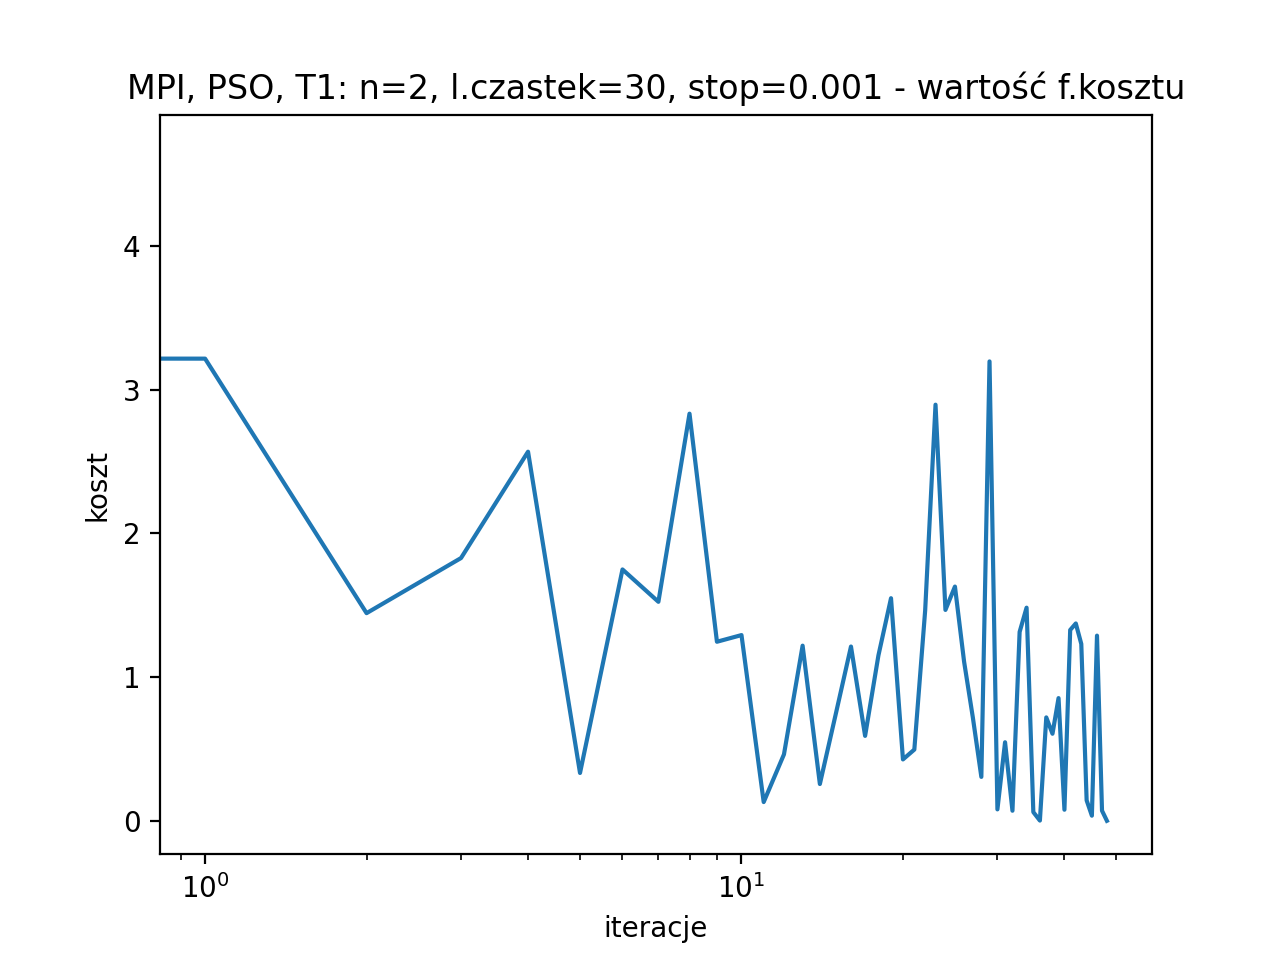
\includegraphics[width=1\linewidth]{grafiki2/MPI_PSO_T1/MPI_PSO_T1_koszt.png}
  \captionof{figure}{Wartość funkcji kosztu dla zadania $1$ dla metody PSO.}
  \label{fig:pozycjeStartowe:PSO1}
\end{minipage} \hfill
\begin{minipage}[b]{\dimexpr.5\textwidth-1em}
  \centering
  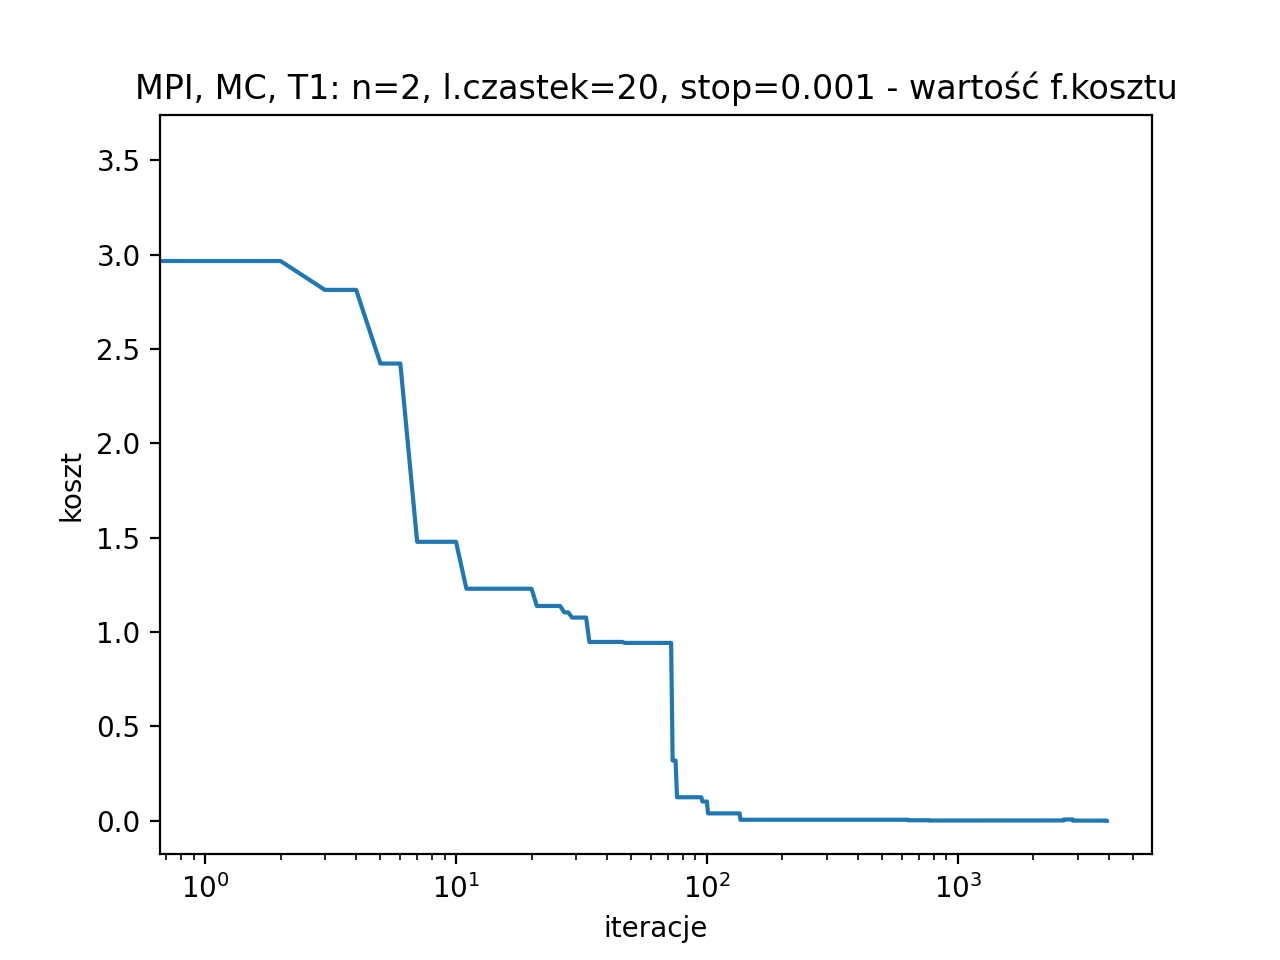
\includegraphics[width=1\linewidth]{grafiki2/MPI_MC_T1/MPI_MC_T1_koszt.png}
  \captionof{figure}{Wartość funkcji kosztu dla zadania $1$ dla metody Monte Carlo.}
  \label{fig:pozycjeStartowe:MC1}
\end{minipage}
\end{figure}

\begin{figure}[H]
\centering
\begin{minipage}[b]{\dimexpr.5\textwidth-1em}
  \centering
  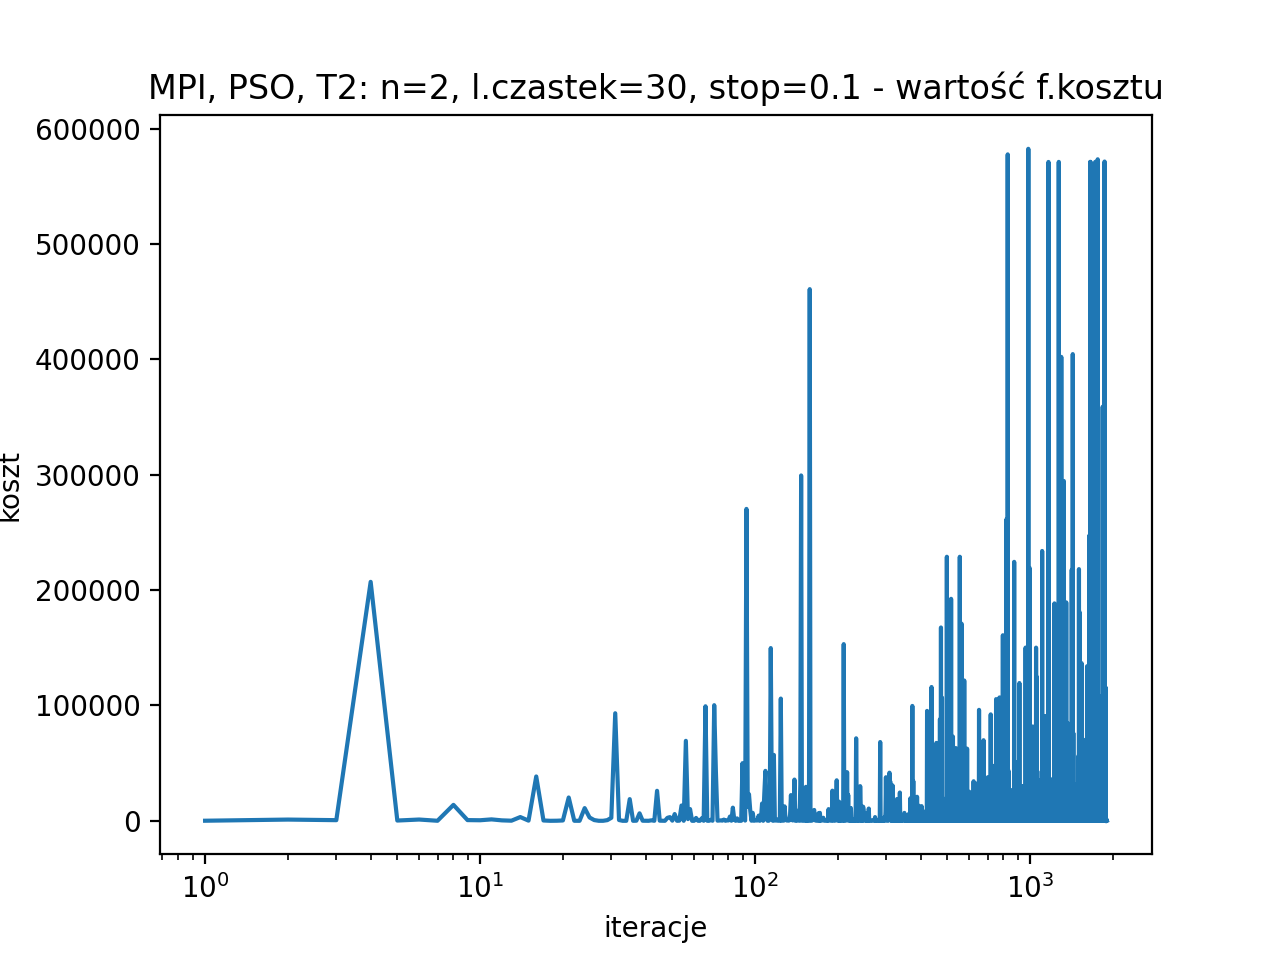
\includegraphics[width=1\linewidth]{grafiki2/MPI_PSO_T2/MPI_PSO_T2_koszt.png}
  \captionof{figure}{Wartość funkcji kosztu dla zadania $2$ dla metody PSO.}
  \label{fig:pozycjeStartowe:PSO2}
\end{minipage} \hfill
\begin{minipage}[b]{\dimexpr.5\textwidth-1em}
  \centering
  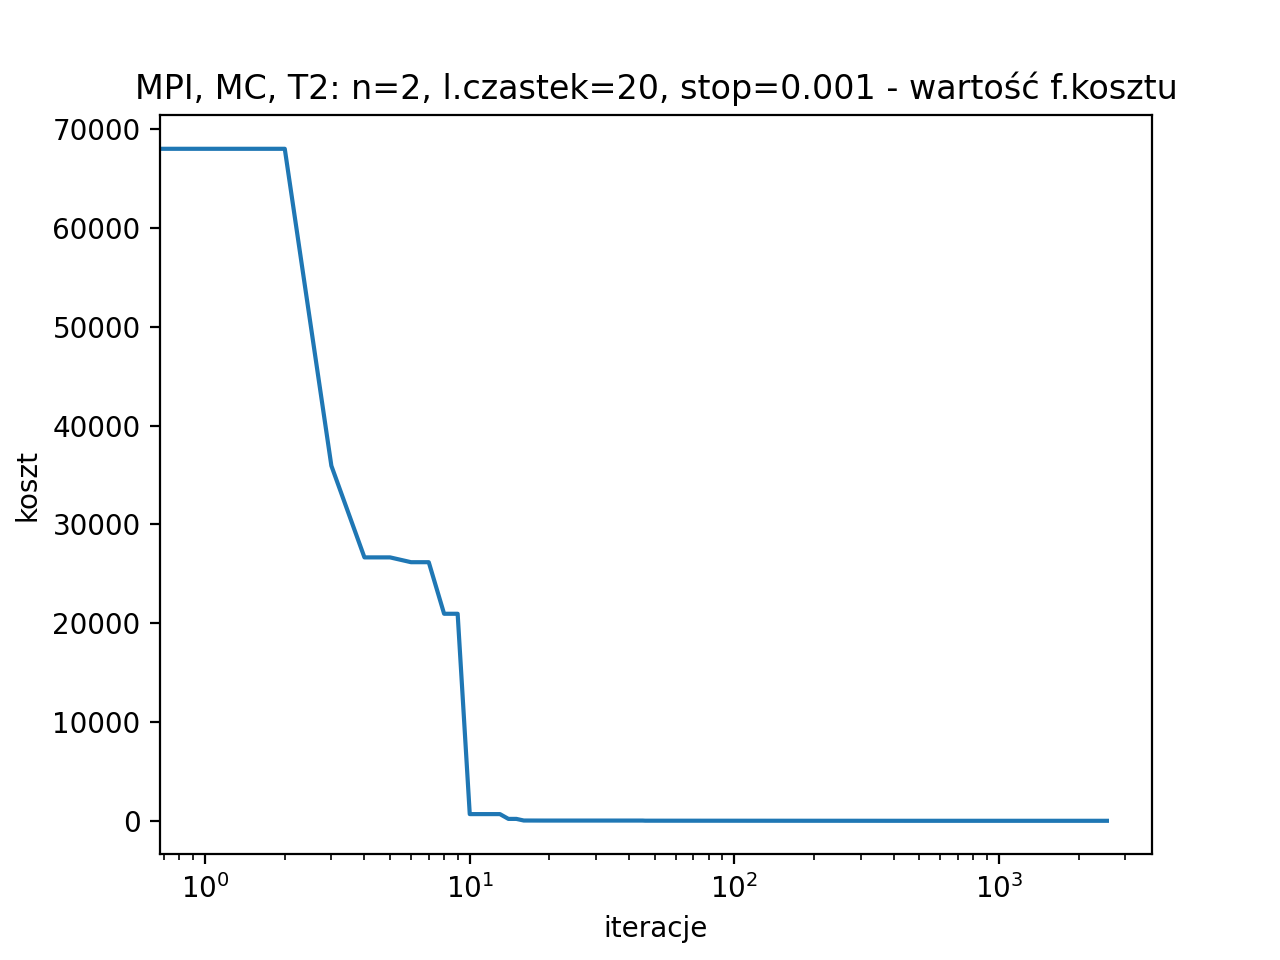
\includegraphics[width=1\linewidth]{grafiki2/MPI_MC_T2/MPI_MC_T2_koszt.png}
  \captionof{figure}{Wartość funkcji kosztu dla zadania $2$ dla metody Monte Carlo.}
  \label{fig:pozycjeStartowe:MC2}
\end{minipage}
\end{figure}

%Pozycje startowe
\begin{figure}[H]
\centering
\begin{minipage}[b]{\dimexpr.5\textwidth-1em}
  \centering
  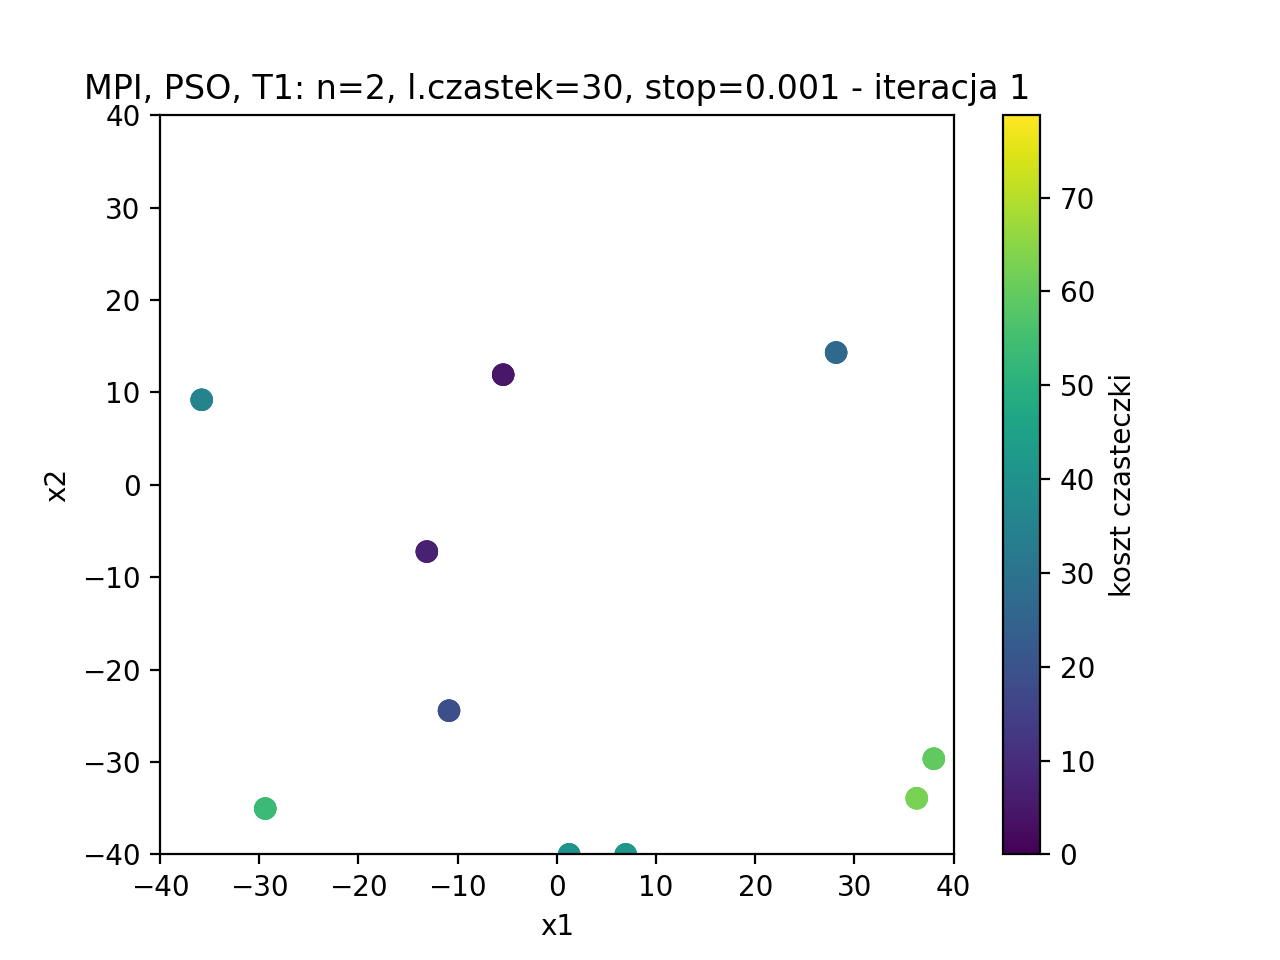
\includegraphics[width=1\linewidth]{grafiki2/MPI_PSO_T1/MPI_PSO_T1_startPositions.png}
  \captionof{figure}{Pozycje startowe cząsteczek dla algorytmu PSO dla zadania $1$.}
  \label{fig:pozycjeStartowe:PSO1}
\end{minipage} \hfill
\begin{minipage}[b]{\dimexpr.5\textwidth-1em}
  \centering
  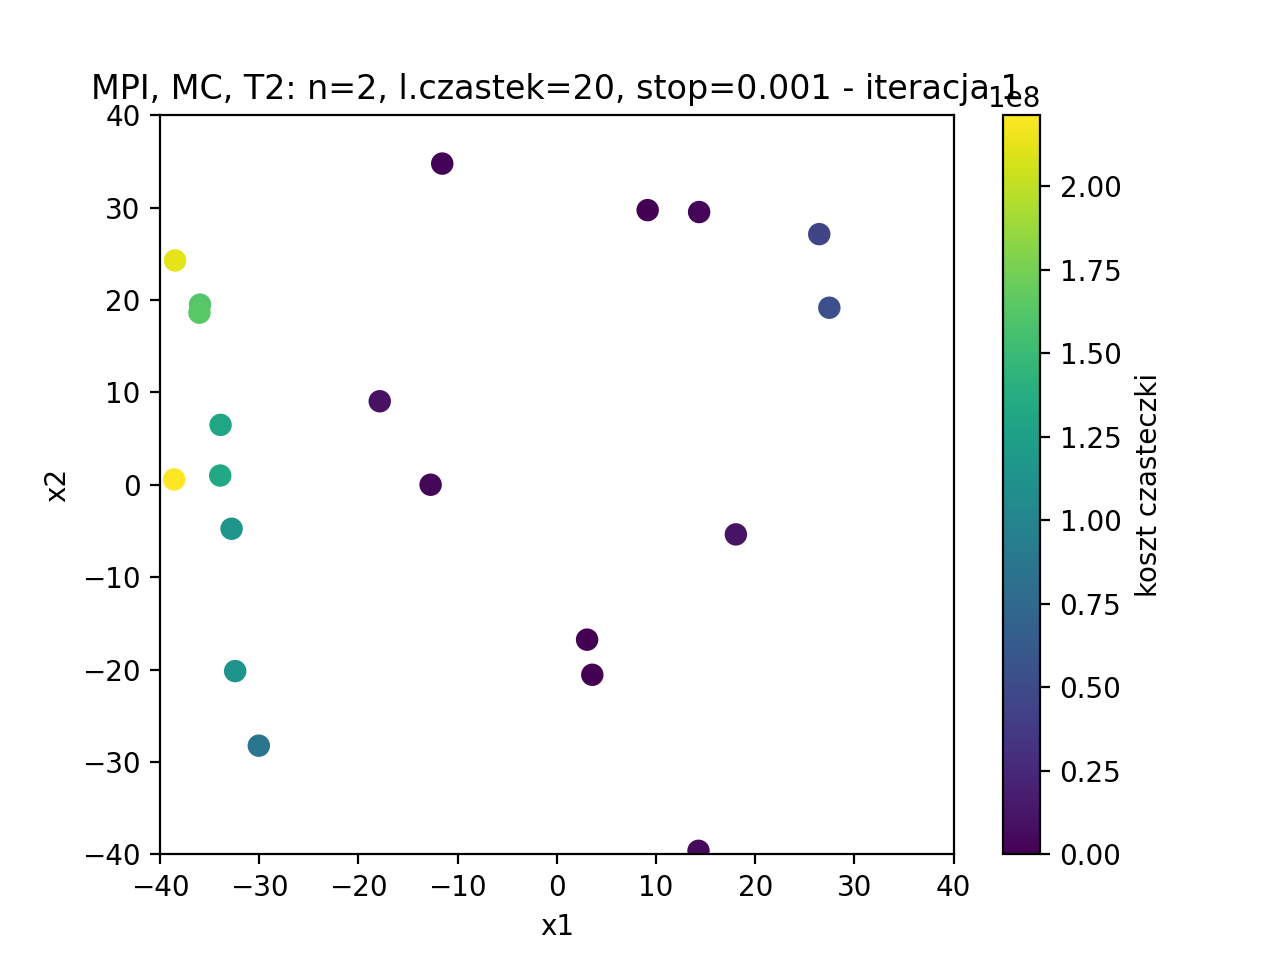
\includegraphics[width=1\linewidth]{grafiki2/MPI_MC_T2/MPI_MC_T2_startPositions.png}
  \captionof{figure}{Pozycje startowe cząsteczek dla algorytmu MC dla zadania $1$.}
  \label{fig:pozycjeStartowe:MC1}
\end{minipage}
\end{figure}

\begin{figure}[H]
\centering
\begin{minipage}[b]{\dimexpr.5\textwidth-1em}
  \centering
  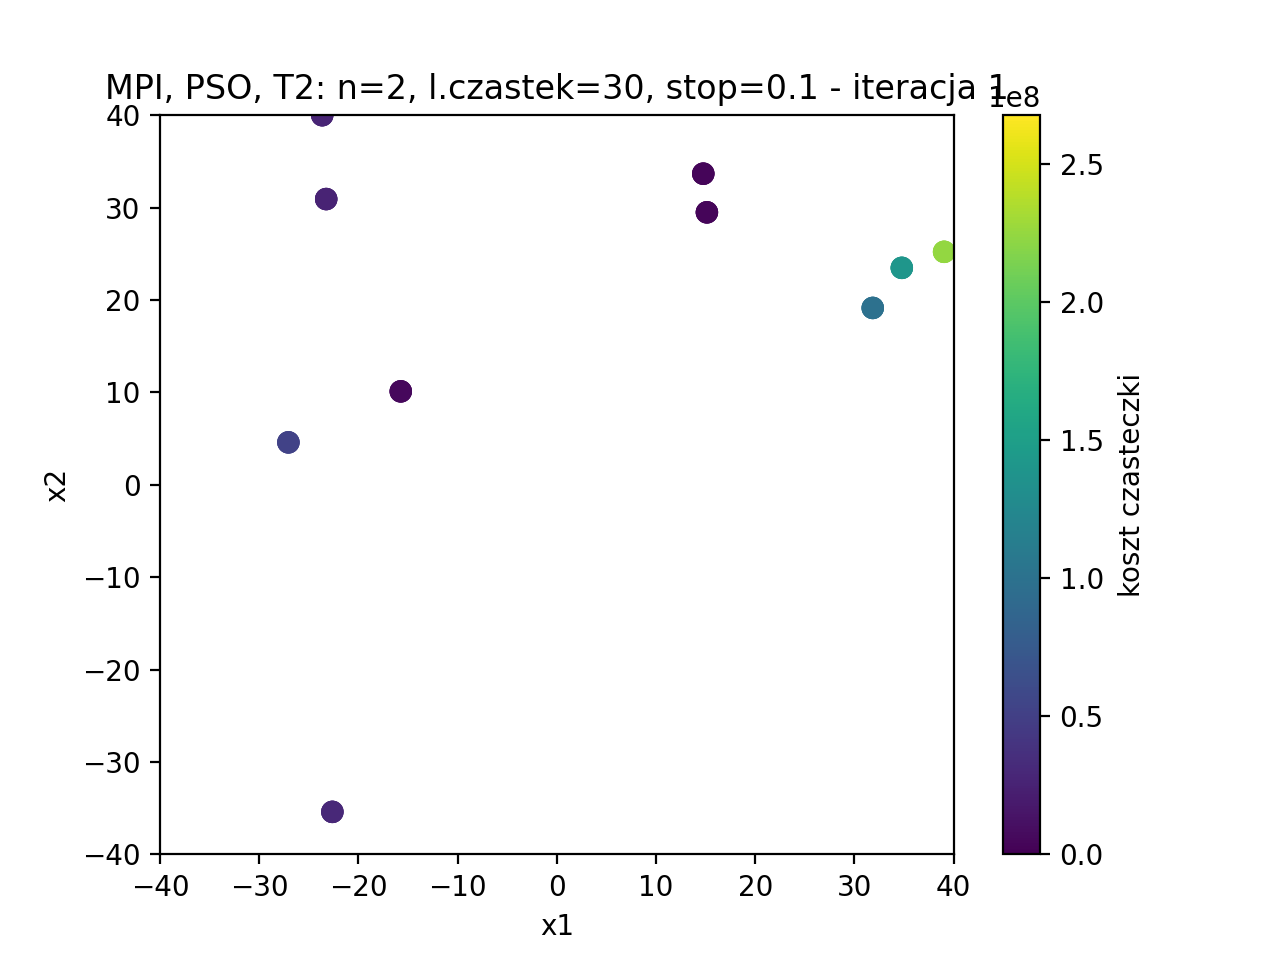
\includegraphics[width=1\linewidth]{grafiki2/MPI_PSO_T2/MPI_PSO_T2_startPositions.png}
  \captionof{figure}{Pozycje startowe cząsteczek dla algorytmu PSO dla zadania $2$.}
  \label{fig:pozycjeStartowe:PSO2}
\end{minipage} \hfill
\begin{minipage}[b]{\dimexpr.5\textwidth-1em}
  \centering
  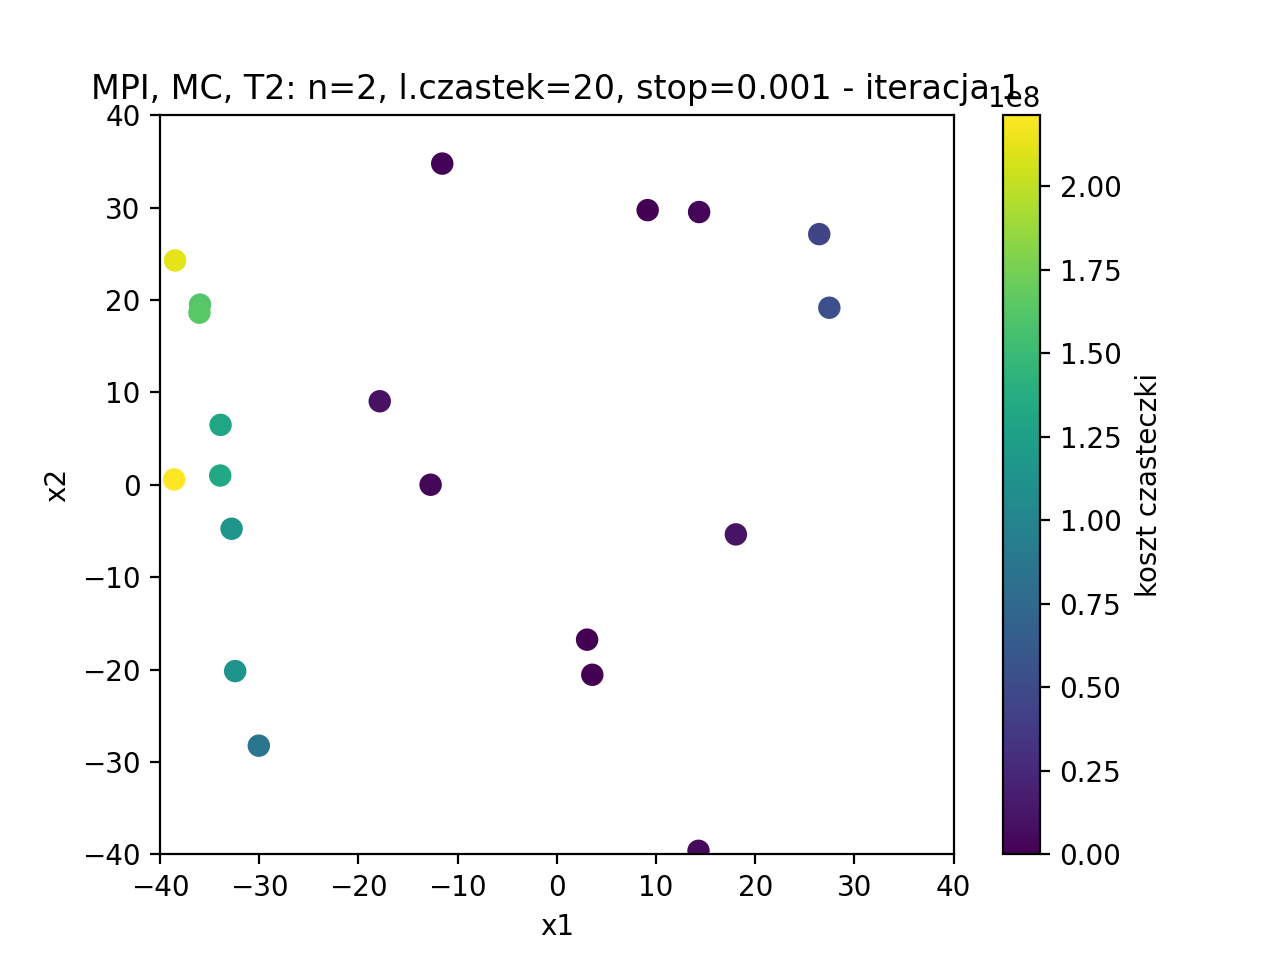
\includegraphics[width=1\linewidth]{grafiki2/MPI_MC_T2/MPI_MC_T2_startPositions.png}
  \captionof{figure}{Pozycje startowe cząsteczek dla algorytmu MC dla zadania $2$.}
  \label{fig:pozycjeStartowe:MC2}
\end{minipage}
\end{figure}



\subsection{Porównanie trajektorii dla $n = 2$ w CUDA}


\section{Wnioski} 



\bibliography{PORR_sprawozdanie_1}{}
\bibliographystyle{plain}

\end{document}







